\documentclass[10pt]{article}
\usepackage[utf8]{inputenc}
\usepackage{graphicx}
\usepackage{multicol}
\usepackage{float}
\usepackage[a4paper,width=150mm,top=25mm,bottom=25mm]{geometry}

\title{
\vspace{-1cm}
{Requirement Analysis}
\item
\begin{figure}[H]
\centering
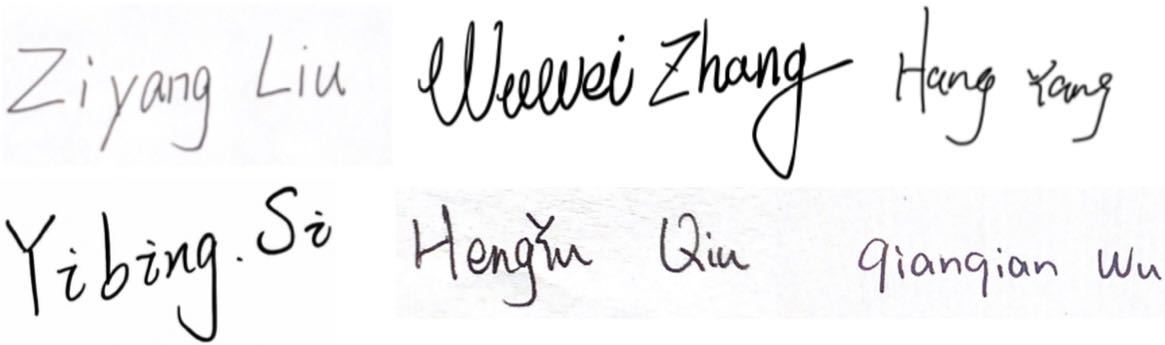
\includegraphics[scale = 0.15]{sign.jpg}
\end{figure}
}
\date{}

\author{COMP208 TEAM39\\Ziyang Liu, Wuwei Zhang,Hang Yang, \\Yibing Si, Hengyu Qiu, Qianqian Wu}


\begin{document}

\maketitle

\section{Mission Statement}
The purpose of our project is to develop a movie website to help users obtain their potential favorite movies based on machine-learning recommendation algorithm which analysis user's preference and behavior, moreover, to build an interest-oriented platform to record, share ideas and communicate with other users.



\section{Mission Objectives}
This web project is designed to satisfy the people's growing demand of watching, sharing movies on personal device in the Covid-19 pandemic setting. Below are our objectives of this system: 
\begin{itemize}
\item Including a fully functional database, and the modified database must save the user's own data and user's preference information.
\item Including a web interface that allows users to use the system (log-in, user preferences and any other services provided to users in the system), and allows administrators to manage the system after authentication.
\item To maintain (input , update and delete) data on users
\item To maintain (input, update and delete) data on user’s current recordings
\item To maintain (input, update and delete) data on user’s histories
\item To maintain (input, update and delete) data on user’s comments
\item To maintain (input, update and delete) data on movie ratings
\item To utilize the recommended algorithm by using machine learning model to analyze both movies' and users' features
\item To provide movie video links which is from streaming media on the movie information page to allow user to access movies
\item To utilize the searching/filter function by query data on movies
\item To perform searches on recipes key words of movies
\item To utilize a login/logout/register function 
\item To utilize a comment function
\item To utilize a scoring and review function
\end{itemize}
According to iMDb, there was around 30 new movies coming out in the United States in December 2020 and it is unnecessary for most people to traverse all. Therefore, our website aims to help and encourage people find and enjoy more movies by reducing the redundant information and making information in order, additionally share their reviews and idea with different people.

\section{System Boundary Diagram}
\begin{figure}[H]
\centering
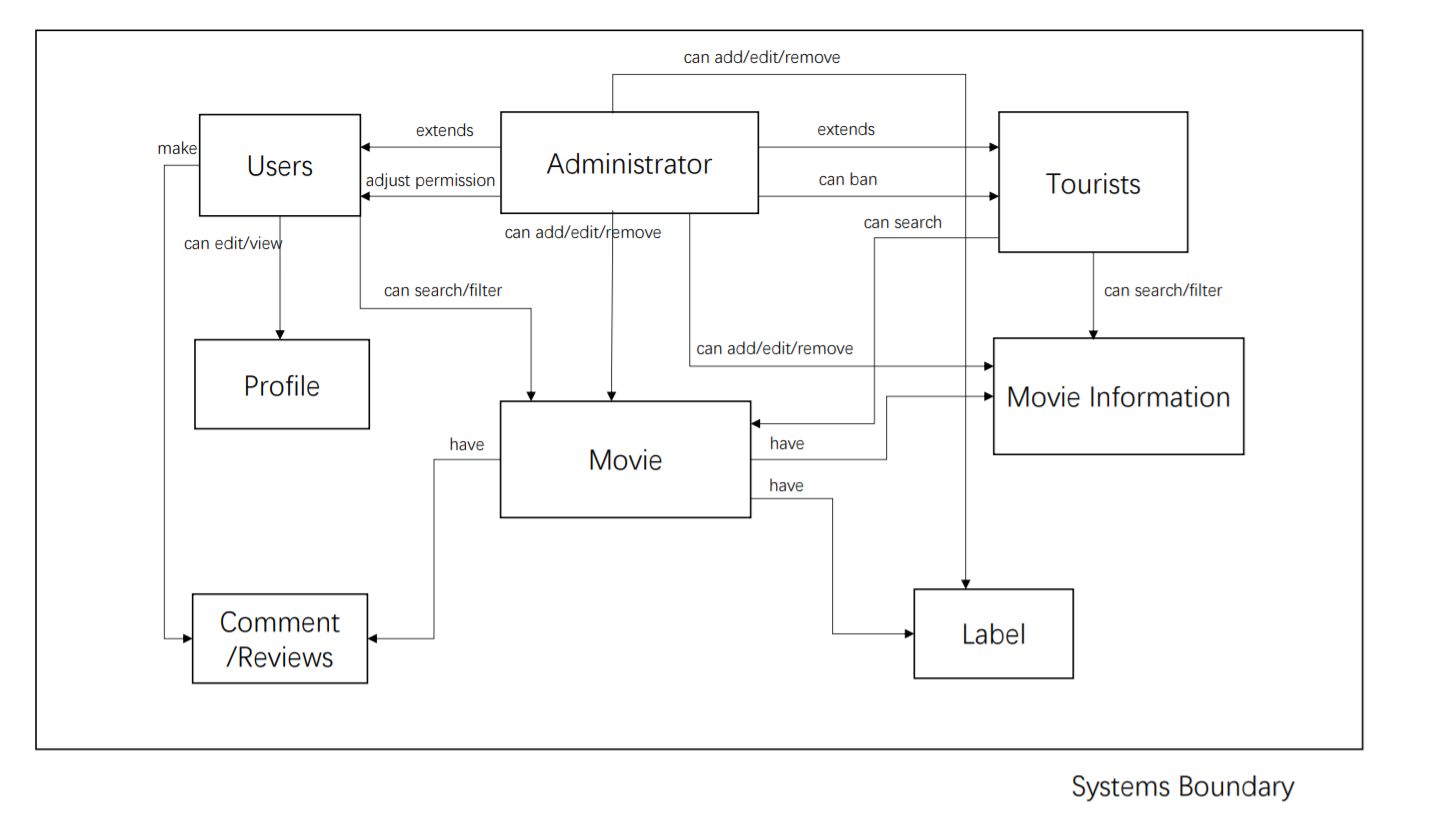
\includegraphics[scale =0.4]{sbd.png}
\caption{System boundary Diagram}
\label{fig:image}
\end{figure}

\section{User Views}
\noindent \textbf{4.1 User: User refer to people who can use all functions on the movie recommendation website after registration.\\}
\noindent 
Once the user log in, they can: 
\begin{itemize}
\begin{multicols}{2}
\item[-] log out.
\item[-] Reset password.
\item[-] Close an account.
\item[-] Edit profile page.
\item[-] Filter by the label.
\item[-] Query operation, enter the name of the movie to search.
\item[-] View the movie information.
\item[-] Score the movies and reviews.
\item[-] Reply to others' movie comment.
\item[-] View other’s profile 
\item[-] If a movie is missing, notify the administrator.
\item[-] Click to enter the movie watching link.   
\end{multicols}
\end{itemize}

\noindent \textbf{4.2 Tourist: Tourist represents people who can use part of the functions on the website without registration.\\}
Tourist do not need to be authenticated, but tourists can also:
\begin{itemize}
\begin{multicols}{2}
\item[-] Register as a user.
\item[-] View the movie information.
\item[-] Filter by the label.
\item[-] Query operation, enter the name of the movie to search.
\end{multicols}
\end{itemize}

\noindent \textbf{4.3 System Administrator: System administrator refers to the staff responsible for the update and maintenance of the movie recommendation system.\\}
once authenticated, they can:
\begin{itemize}
\begin{multicols}{2}
\item[-] Update the film.
\item[-] Update the label.
\item[-] Increase or decrease user permissions.
\item[-] Maintains the database: views, adds, modifies, deletes records.
\item[-] Maintain code and handle potential program damage.

\end{multicols}
\end{itemize}

\begin{figure}[H]
\centering
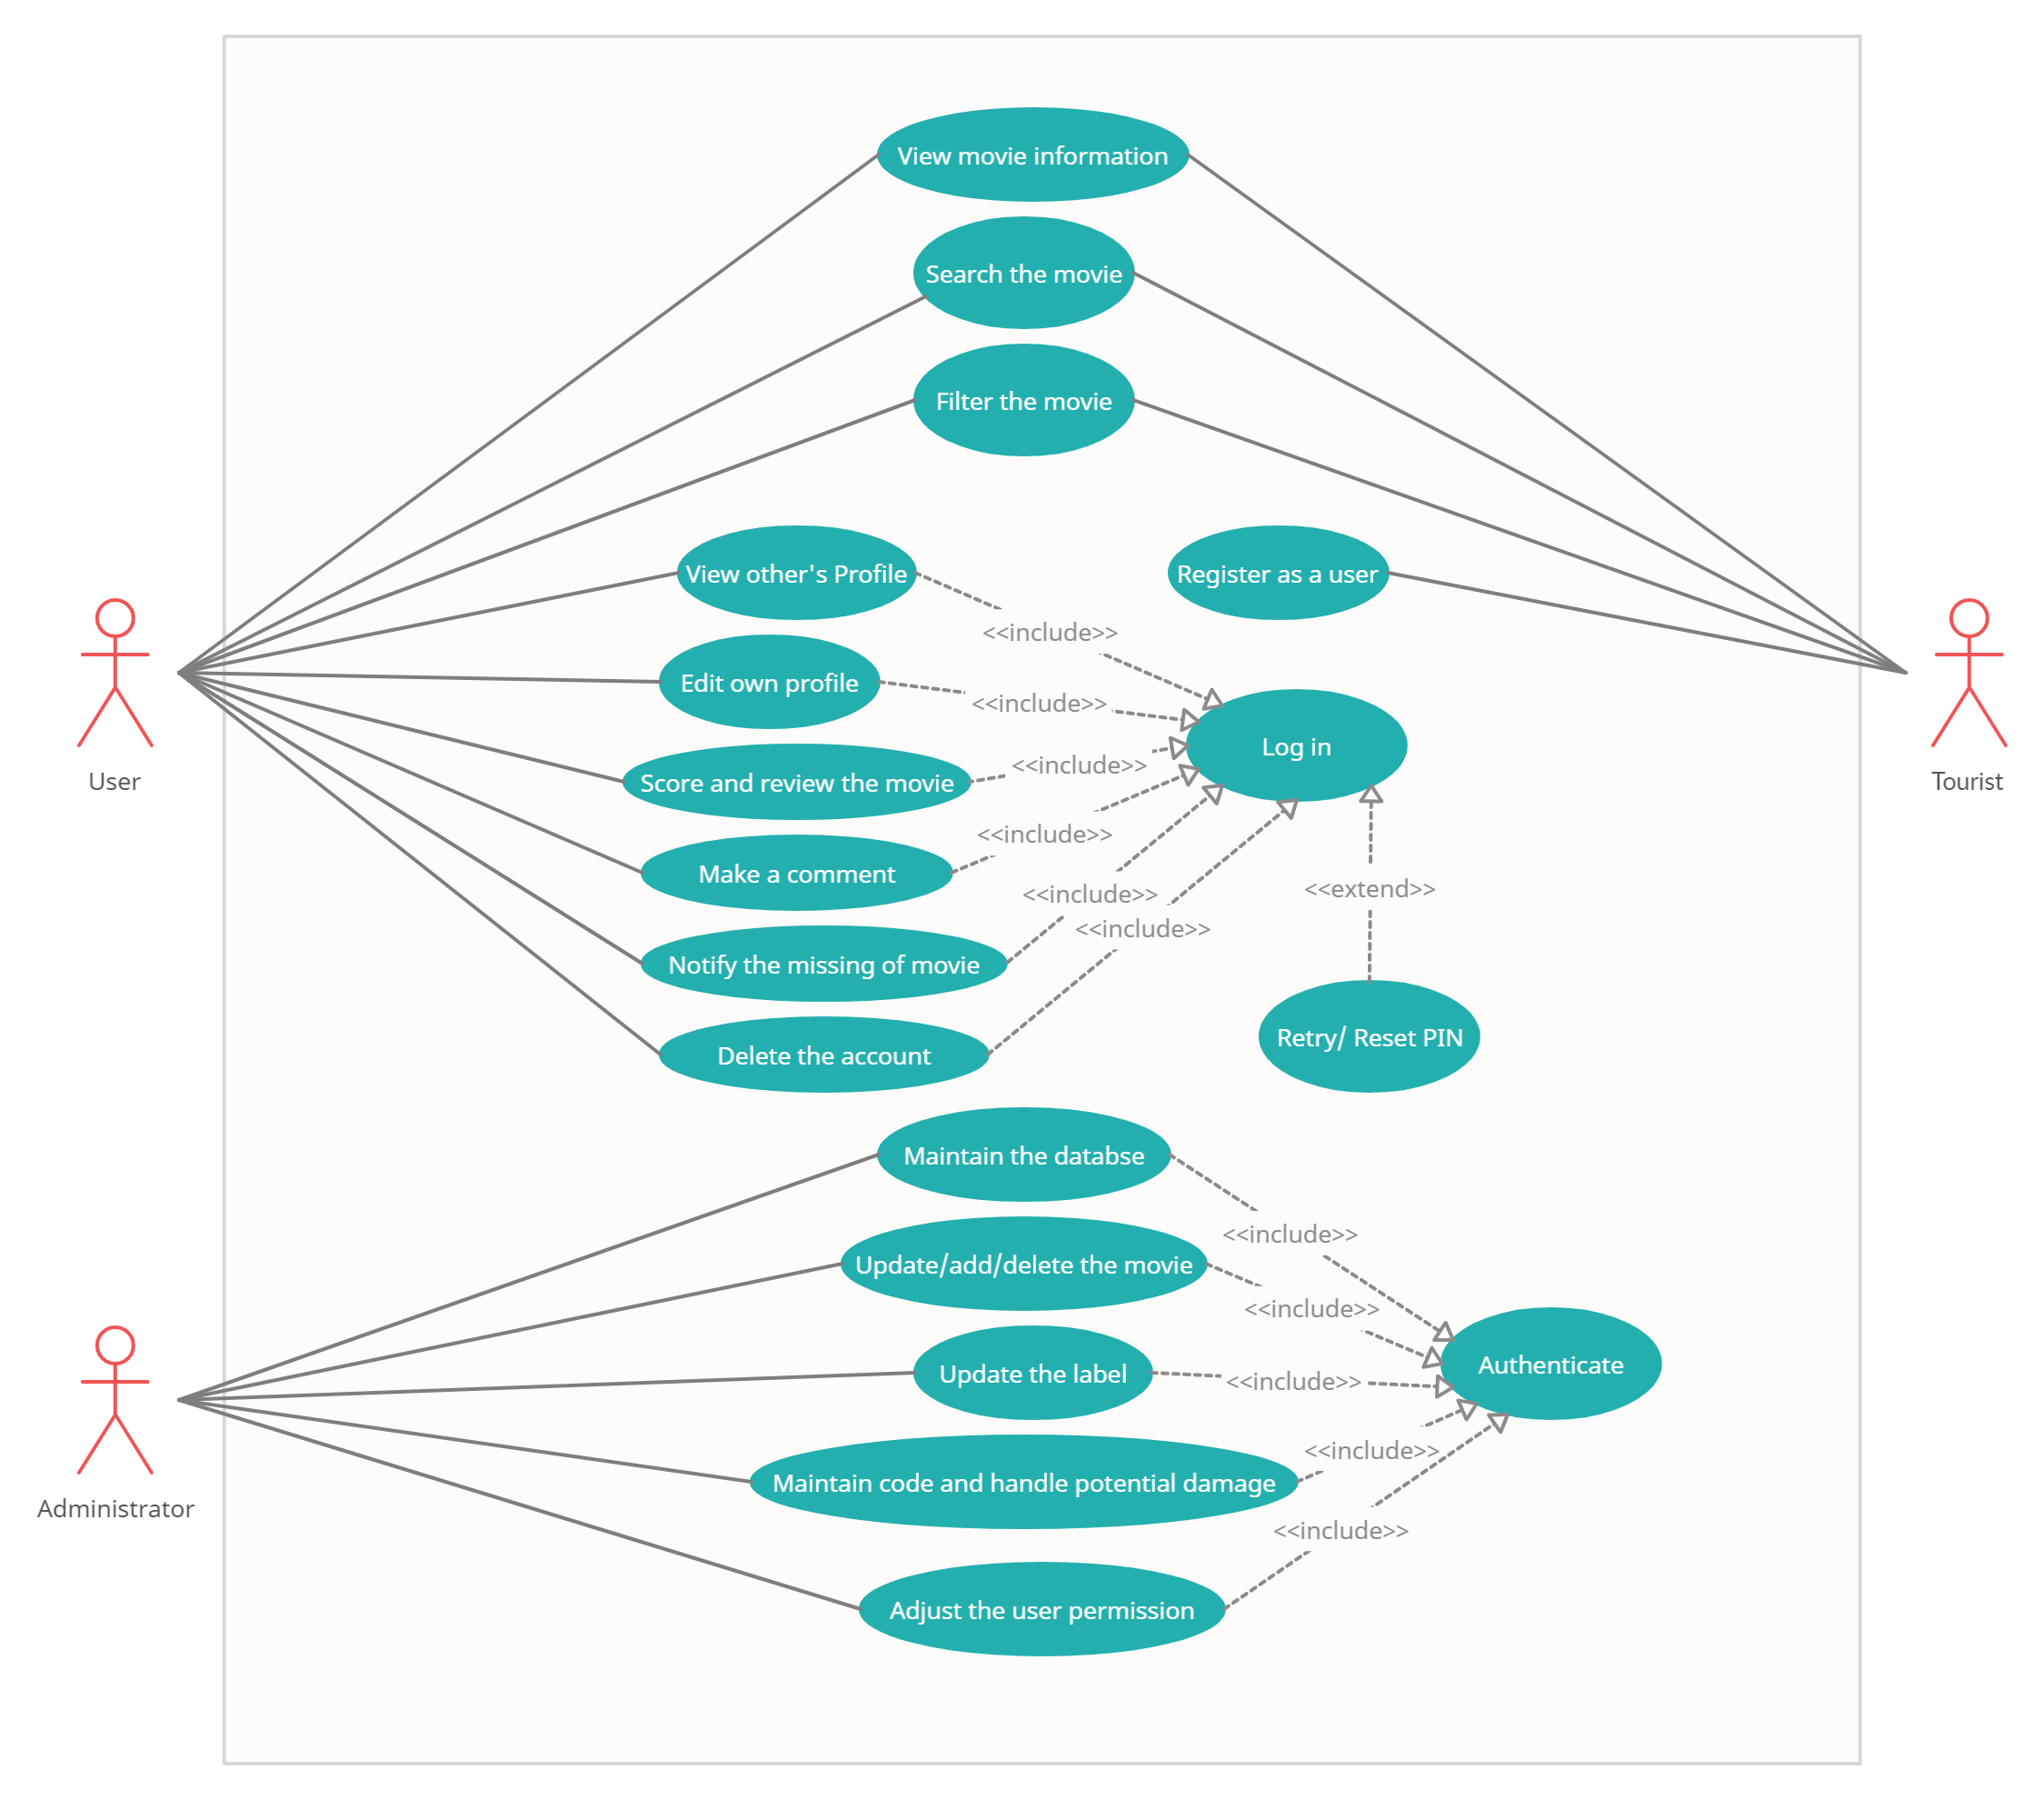
\includegraphics[scale =0.188]{UCD.png}
\caption{Use Case Diagram}
\label{fig:image}
\end{figure}


\section{Transaction requirements}
\subsection{Data Entry}
\begin{multicols}{2}
\noindent 
- Entry the information of a new movie\\
- Entry the comments of a movie\\
- Entry the username and password of a new user\\
- Entry the score of a movie\\
- Entry the key word of a movie\\
- Entry the watch link of a movie\\
\end{multicols}
\subsection{Data Update}
\begin{multicols}{2}
\noindent
- Update the password of a user\\
- Update the amount of accounts\\
- Update the comment of a movie\\
- Update the score of a movie\\
- Update the watch link of a movie
\end{multicols}
\subsection{Data Queries}
\begin{multicols}{2}
\noindent
- Queries the information of a account\\
- List the the result of the query for the keyword\\
- List the comment of a movie\\
- List the score of a movie\\
- List the dialogues between two user\\
- List the label of personalized recommendations\\
\end{multicols}


\section{System Requirements}
\noindent
\textbf{Initial Database Size\\}
- The database must be able to hold records for at least 50 users, 4000-6000 movies and 100 reviews, comments for each movie

\noindent 
\textbf{Rate of Growth \\}
- The database must have the capability to expand as user’s information, movies’ information are added to the system.\\
- The recommendation model must have ability to update and improve it's prediction as new user’s information, movies’ information are added to the system.

\noindent 
\textbf{Expected type and frequency of searches\\}
- Both tourists and users frequently search for movies and browse the movie information which is from the database by keywords our using filter\\
- A large number of registered users frequently record their comments and ratings through the database\\
- The recommendation model will frequently analyze and recommend the movie as new user’s information, movies’ information are added to the system.

\noindent \textbf{Network and Access requirements\\}
- Constant database access will be required for the system to retrieve the user’s data and movies’ data\\
- Registered users and tourists have different permissions, such as registered users can comment and score the movie while visitors can't. \\
- System administrators have the highest privileges to delete comments, modify movie information, and reset user passwords.

\noindent \textbf{Performance\\} 
-The system is able to respond effectively to a user's request within 30 seconds

\noindent \textbf{Security\\} 
- The system will require 3 levels of hierarchy; system administrators, registered users and tourists.\\
- as system administrators and registered users, each user will have login details consisting of a ‘User ID’ and a password. \\
- Each password must contain at least 8 characters and at least 1 number. 
- All passwords in the database are stored as hashes. \\
- System administrators will be at the top of the hierarchy and can perform the highest level tasks such as selecting the project managers. System 	administrators can also perform all the tasks that the project managers can.

\noindent \textbf{Backup and Recovery\\} 
- In the event that a user forgets their password, system administrators can reset their password to a default value. \\
- If a system administrator forgets their password, the password will have to be 
manually reset from within the database on the developer’s end. \\
- If the system crashes, use the backup and rollback of the database to recover the database.

\noindent \textbf{Legal Issues\\} 
- The system and the data held within the system must be in compliance of the UK Data Protection Act 1998.

\section{Project planning}
As lots of film recommendation system in service, we plan to design a more GUI-friendly web and advanced recommendation algorithm to support the system.\\
We chose to be using Agile methodology for developing software. Agile development make our project has the advantages of adaptive planning, evolutionary development, early delivery, and continual improvement.\\The task and code will be developed modularly, which means they’re easy to manage and we can work on different task simultaneously. \\At last, our project will be using GitHub as the host platform for version control and collaboration.
%
%\subsection{Project Scheduling}
%\begin{figure}[H]
%\centering
%\includegraphics[scale =0.8]{sc3.jpg}
%\end{figure}
%
\begin{figure}[H]
\centering
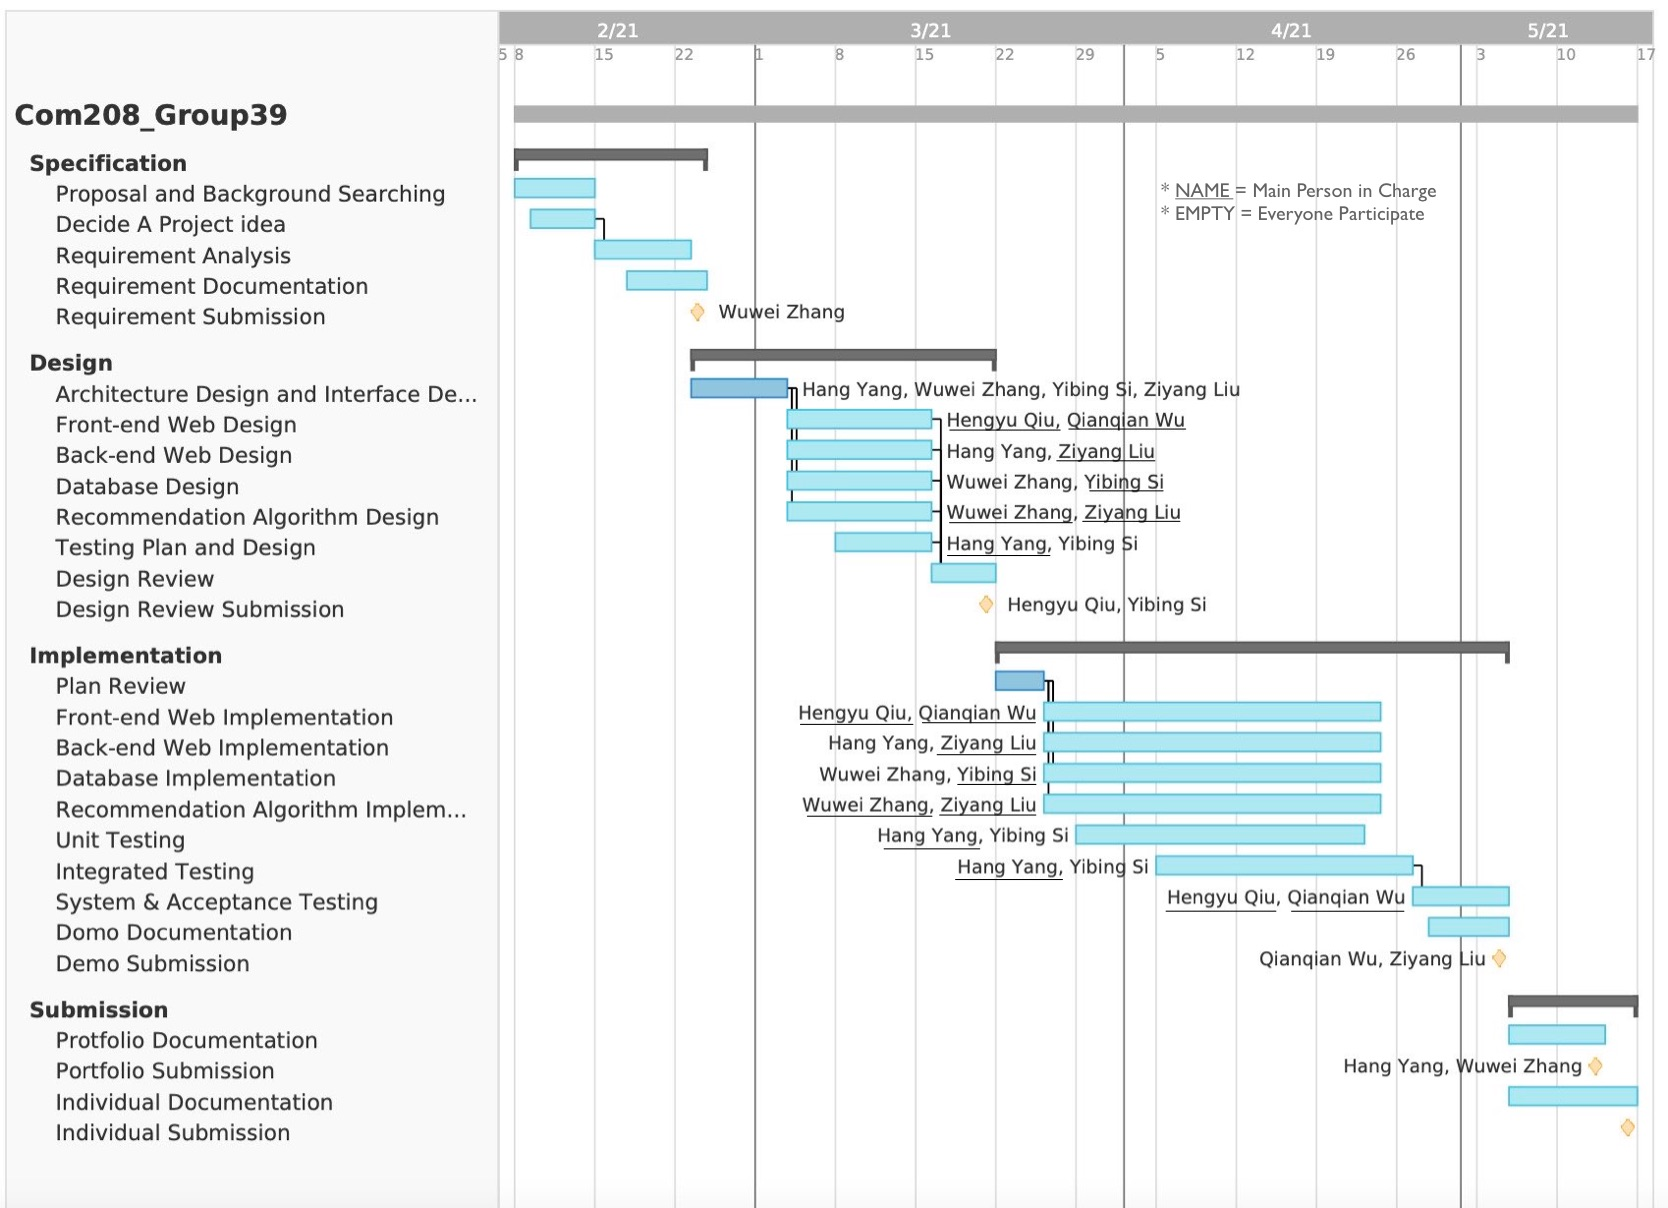
\includegraphics[scale =0.26]{GTD.jpg}
\caption{Gantt Diagram}
\label{fig:image}
\end{figure}


\subsection{Risk Management}
\subsubsection{Risk Analysis}
- Producing the algorithm efficiently especially for cold start problem is quite tricky, and optimizing the recommendation algorithm to provide the best related films to users is also considered a main issue for algorithm implementation.\\
- Sets of new skill required, teams must learn and Implement over very short periods of time.\\
- Requirement document might be incomplete.\\
- Members are delaying delivering code for testing.\\
- Two of project members are outside the UK, it’s impossible to host a efficient face-to-face communication. 
\subsubsection{Risk plan}
- Progress report during very project meetings is required, and every task leader have to check Gantt chart frequently, set deadline for each task members. \\
- Allocating more tests for High-risk areas and less tests for medium and low-risk regions.\\
- Lots of time are assigned to submission stage(as show in fig.assignment chart) to avoid system testing error and refine the project. 


\section {References}
\noindent [1] "- IMDb", \textit{IMDb}, 2021. [Online]. Available: https://www.imdb.com/. [Accessed: Feb- 2021]\\
\noindent [2] I. Sommerville, \textit{Software engineering.} Boston: Pearson, 2011.\\


\end{document}
